\documentclass[hidelinks, 12pt, a4paper]{article}

\usepackage[utf8]{inputenc}
\usepackage[margin=1.5cm]{geometry}
\usepackage{graphicx}
\usepackage{setspace}
\usepackage[T1]{fontenc}
\usepackage{tocloft}
\usepackage{todonotes}
\usepackage{epstopdf} 
\usepackage{hyperref}
\usepackage{float}
\usepackage{titlesec}
\usepackage{listings}
\usepackage{multirow}
\usepackage{xcolor}
\usepackage{mwe}
\usepackage{hyperref}
\onehalfspacing
\usepackage[english]{babel}
\usepackage{fancyhdr}
\usepackage{enumitem}

\pagestyle{fancy}
\fancyhf{}
\rhead{blulancetech@gmail.com}
\lhead{Carpool}
\rfoot{Page \thepage}

\author{}
\date{}
\title
{
	
\includegraphics[width=6cm]{images/up_logo.jpg} \\
	Department of Computer Science \\
	Faculty of Engineering, Built Environment \& IT\\
	University of Pretoria \\
	\vspace{0.5cm}
	\Huge COS301 -
	Software Engineering\\
	\vspace{1cm}
	{\Huge Carpool}\\
	\begin{Large}
		Software Requirements and Design Specifications
	\end{Large}
	\vspace{0.5cm}
	
    \begin{center}
    \noindent
    
\includegraphics[width=6cm]{images/company_logo.png} 
    \vspace{0.5cm}
    \begin{table}[h]
    \centering
    \begin{tabular}{|l|l|l|}
    \hline
    Name  & Student Number\\ \hline
    Benjamin Osmers & u16068344 \\ \hline
    Ashleigh Govender &  U20528834      \\ \hline
    Joshua Brink  & U19185678 \\ \hline
    Jason Antalis     & U19141859     \\ \hline
    Wesley Pachai & U20578688    \\ \hline
            
    \end{tabular}
    \end{table}
    \end{center}
    }
% \setlength {\marginparwidth}{2cm}
\begin{document}
\maketitle


\newpage
\tableofcontents 
\newpage
\section{Project Information}
    
        \qquad \textbf{Project Name:} 
        
           \qquad  \qquad Carpool\\
        
        \textbf{Owner Contact Details:}

          \qquad  \qquad Matthew Wood \qquad \qquad \href{matthew.wood@advance.io}{matthew.wood@advance.io} \qquad \qquad
          
           \qquad  \qquad Keegan Ferrett \qquad \qquad \href{keeganf@mit.edu}{keeganf@mit.edu}\\
           
           
                   \textbf{Lecture mentor:}

          \qquad  \qquad David  \qquad \qquad \href{matthew.wood@advance.io}{matthew.wood@advance.io} \qquad \qquad
          
          	\vspace{1.5cm}
          	
\section{Introduction}
Carpooling is a method of sharing unoccupied seats in a car with people who commute along the same route. Usually, one person from the group drives their personal car and the others all share the cost of the trip. Due to the environmental crisis that the world faces, carpooling has become immensely popular as it reduces the number of cars on the road. Of recent carpooling has become the latest trend as petrol prices continue to increase. Carpooling has evolved into a viable, cost-effective, and stress-free mode of transportation. Finding individuals to carpool with is challenging, since it is difficult to locate someone travelling to the same destination at the same time as you. This Carpool application is a solution to this problem. \\ \\
Carpool is a mobile application that helps students find affordable transport to and from campus or longer trips such as returning home for semester break. Carpool provides students with a central location whereby they can post, find, and join safe car trips. This application allows students with vehicles to save on petrol costs as well as provide affordable transportation to students who do not have vehicles. Students can travel to their desired location while sharing the car and expenditures.\\ \\
\textbf{Vision:}\\
A more affordable and practical version of Uber/Lyft for students. Students can be both drivers and passengers.\\ \\
\textbf{Objective and Scope:} \\
To create an Android and IOS mobile application for students, whereby they are able to post, find and join safe car trips with ease.

\newpage
\section{Users}

\subsection{User Characteristics}
    
The user should have the ability to operate and own a mobile device such as a smartphone or tablet. The user should have constant access to the internet and location services to download and utilize the Carpool application. The following are users of the Carpool System:\\
    
    \Large{ \textbf{Admin} }
    \normalsize
        \begin{itemize}
            \item A person who manages the Carpool system
            \item A person who verifies a user’s email address and driver’s license.
            \item 	A person who manages the users
            \item 	A person who does maintenance and routine checks on the system
            \item 	A person who can help users with the functionality and navigation of the system

        \end{itemize}
    
    \vspace{0.5cm}
    \Large{\textbf{User}}
    \normalsize
    
    Students will be the main users of the application and will be verified through their university email. Students can be broken up into two categories namely Passengers and Drivers.\\
    
    \large{ \textbf{General} }
    
        \begin{itemize}

            \item A person who has access to a smart device that has location and internet services.
            \item A person that is studying at a recognised university in South Africa.
            \item A person who is able to share their locational services.
            \item A person who can communicate with other users through the chat functionality on the platform.
            \item A person who does not mind sharing their journey with other people.
            \item A person who can view other user's profile.
            \item A person who can use the map services provided by the platform.
        \end{itemize}
        \vspace{5.0cm}
        
    \large{ \textbf{Driver} }
    
        \begin{itemize}

            \item A person who is 18 years and older and has a valid driver license.
            \item A person who owns/ has access to a road worthy vehicle.
            \item A person who wants to Create Trips.
            \item A person who can decline or accept users that book seats.
            \item A person who can cancel trips that they have created.
            \item A person who is responsible for starting and ending trips.
            \item A person that can send reminders and information about the trip to users on the trip.
            \item  A person who is responsible for picking up and dropping off passengers at their location.
        \end{itemize}
        \vspace{0.5cm}
        
            \large{ \textbf{Passenger} }
    
        \begin{itemize}

            \item A person who can search and book trips.
            \item A person who owns a credit card and can afford to book a trip.
            \item A person who can rate their trip experience.
            \item A person who can decline or accept users that book seats.
            \item A person who can cancel trips that they have created.
            \item A person who is responsible for starting and ending trips.
            \item A person that can send reminders and information about the trip to users on the trip.
            \item  A person who is responsible for picking up and dropping off passengers at their location.
        \end{itemize}

    \newpage
\subsection{User Stories}
 \begin{changemargin}
    \begin{itemize}
        \item \textbf{\underline{User Story 1: }}\\
        As an Admin I want to verify a student's email address and driver license, so that only valid users can access the application (Students who study at a recognized University in South Africa).
        \item \textbf{\underline{User Story 2: }} \\
        As an Admin I want to review user's reviews so that I can prohibit users who have bad ratings
        \item \textbf{\underline{User Story 3: }} \\
        As a user I want to be able to login to my account and change my personal details on my profile such as (profile picture, name, surname, email, banking details and contact number).
        \item \textbf{\underline{User Story 4: }} \\
        As a User I want to view my previous trips so that I can have a record of all User I have been in contact with and view my previous destinations.
        \item \textbf{\underline{User Story 5: }} \\
        As a driver I want to be able to create my own trip by posting the date, seats available, price per seat, starting location and destination of the trip. This will help me find individuals to carpool with. I would also like to edit and delete said trips.
        \item \textbf{\underline{User Story 6: }}\\
       As a driver I want to be able to accept or decline passengers that can book a seat on my trip, this ensures that I am comfortable with those that are sharing the journey with me.
        \item \textbf{\underline{User Story 7: }} \\
        As a driver I want to receive income from my trips so that I can pay for the costs occurred on the trip (petrol).
        \item \textbf{\underline{User Story 8: }} \\ 
        As a driver I want to be able to send messaged to Passenger so that I can communicate with them information about the trip. I want to be able to communicate with them all at the same time and not send messages to them individually.
        \item \textbf{\underline{User Story 9: }}: \\
       As a Passenger I want to be able to view all trips that have been recommended to me based on my current location and previous trips so that I can pick the most suitable trip to join at ease.
        \item \textbf{\underline{User Story 10: }} \\
       As a Passenger I want to be able to enter my start and destination location in order to find trips that match my specification.
        \item \textbf{\underline{User Story 11: }} \\
       As a Passenger I want to be able to rate my trip experience so that future passengers can get insight on the driver and their trips.
        \item \textbf{\underline{User Story 12: }} \\
        As a Passenger I want to be able to view driver's ratings allowing me to join trips with higher ratings (small chance of something going wrong on the trip if a driver has a high rating).
        \item \textbf{\underline{User Story 13: }} \\
       As a budget-conscious driver  I'd like to spend less money on my commute so that I can pay off other monthly expenditures. 
        \item \textbf{\underline{User Story 14: }} \\
        As an Environmental activist user. I'd like to reduce the number of cars on the road so that I can play my part in reducing the world’s carbon footprint.
        \item \textbf{\underline{User Story 15: }} \\
        As a women user, I want a method of transportation that I can trust so that I do not have to worry about my safety as a woman.
        \item \textbf{\underline{User Story 16: }} \\ 
        As a student with a limited budget user, I want an inexpensive way to travel so I don't have to rely on public transportation.
        \item \textbf{\underline{User Story 17: }} \\ 
        As a commuter on a long route, I wany to be able to chat to someone so that the travel feels shorter.
        
        
    \end{itemize}
  \end{changemargin}
  
  \newpage
\section{Functional Requirements}

    \begin{changemargin}
    
        \subsection{Must-have requirements}
            \begin{enumerate}[.9in,label=R.\arabic*]
    
                \item The system must provide users with the opportunity to create and manage their accounts.
                \item The system must provide users with the opportunity to Login.\\
                R2.1 If the user forgets their password, the system must allow the user to change their password in a   secure manner.
                
                \item The system must verify the user.\\
                R3.1: The system must verify that the user is a student by verifying their university email.\\
                R3.2  If the user is a driver, The system must verify the user's driver license.

                \item The system must provide the user with the opportunity to create and post trips.\\
                R4.1: The system must allow users to cancel these created trips.\\
                R4.2: The system must allow users to edit these created trips.\\
                R.4.3: The system must notify drivers when these created trips are fully booked.\\
                R4.4: The system must allow the user who created the trip to accept or decline users who book available seats.\\

                \item The system must allow users to browse trips that have seats available.
                \item The system must provide users with the opportunity to book a seat on an available trip.
                \item The system must provide a search functionality for trips using a variety of search criteria (drivers, location, price).
                \item The system must allow a user to view other users’ profiles.
     \newpage           
        \subsection{Could-have requirements}

                \item The system must allow users to make secure online payments for their trips.
                \item The system must allow users to rate fellow carpoolers after a trip.
                \item The system must have a route history for users to view.
                \item The system must have a secure real-time chat feature.
                
        \subsection{Nice-to-have requirements}
        
                \item The system must have an integrated tracking feature.
                \item The system must recommend trips to the user based on their current location or their previous trip history.
                \item The system must allow users to set emergency contacts and send these contact notifications/updates.
                \item The system must allow users to send and receive notifications about trips (reminders).

            \end{enumerate}
            
    \end{changemargin}
    
    \newpage
\section{Quality requirements}

    \begin{changemargin}
    \large{ \textbf{Scalability}}
        \begin{itemize}
            \item[-] Currently the carpool application is only for students in South Africa but it could be expanded internationally. 
            \item[-] As the number of users and operations grows, the server and database must be able to scale both vertically and horizontally.  The system must be able to accommodate a user base from 100 users to 1 million users.
          \end{itemize} 
\vspace{0.5cm}
    \large{ \textbf{Performance}}
            \begin{itemize}
             \item[-] The database must function well in order for the user to have no delays in the program. 
             \item[-] Reading is more significant than writing since users are more likely to spend time browsing than posting trips. As a result, few actions write to the database. Hence a read operation should take less than 500ms and a write operation should approximately 1s.
             
             \end{itemize}
\vspace{0.5cm}
    \large{ \textbf{Security}}
         \begin{itemize}
            \item[-] Because users' passwords and banking details  are kept in the database, the database must be encrypted in order to safeguard this data. 
            \item [-] Because users' passwords and banking details  are kept in the database, the database must be encrypted in order to safeguard this data. 
        \end{itemize}
\vspace{0.5cm}    
    \large{ \textbf{Maintainability}}
         \begin{itemize}
            \item[-] The system should be maintainable in the future.
            \item [-] The system should be well documented such that that new developers can quickly comprehend  the system.
            \item[-] We should be certain that the technology we choose will be supported for a long time.
            \item [-] It should be simple to add new functionality to the system or alter existing functionality. The system should be decoupled as much as possible.
            \item[-] All modifications should adhere to the system's current coding standard, ensuring that the modified system is indistinguishable from the original.
            \item [-] Admin users should be able to track performance, allowing the system's owner to make well-informed judgments about whether or not the system's capacity should be raised.
            \item[-] The system should be checked and maintained on a regular basis, at least twice a month. Users should be informed about this maintenance at least 24 hours ahead of time so that they may make the required preparations.


        \end{itemize}
    \end{changemargin}
\vspace{0.5cm}    
    \large{ \textbf{Usability:}}
            \begin{itemize}
             \item[-] The system should be simple and intuitive to use, making use of the recognition over recall concept. 
             \item[-]The user should be able to see the system's responses, whether favorable or negative. These responses should contain enough information, allowing the user to know exactly what went wrong or right.
            \item[-] Buttons and instructions should be placed in a basic and straightforward manner.
            \item[-]Buttons, graphics, and text should be made large enough to improve clarity, user comfort, reduce annoyance, and reduce the chance of selection mistakes.
            \item[-]The navigation of the application should be kept simple, ensuring all users are able to navigate through the application at ease.
            
             \end{itemize}
 \vspace{0.5cm}            
        \large{ \textbf{Reliability:}}
            \begin{itemize}
             \item[-] The software should be extremely reliable. If a crash occurs, the system should be able to offer sufficient information as to why the crash happened, allowing us to swiftly correct the problem.
             \item[-] Each component of the system should perform as the developers planned.
             \item[-] Before being released to the public, the system should be fault tolerant and properly tested.
             \item[-] 	The system should be operational 99.9\% of the time.

             \end{itemize}


\newpage
\section{Class Diagram}
The connection between the various subsystems and their individual classes are depicted in depth in Carpool’s class diagram.
\vspace{1.5cm}
    
        \begin{figure}[H]
        
            \centering
            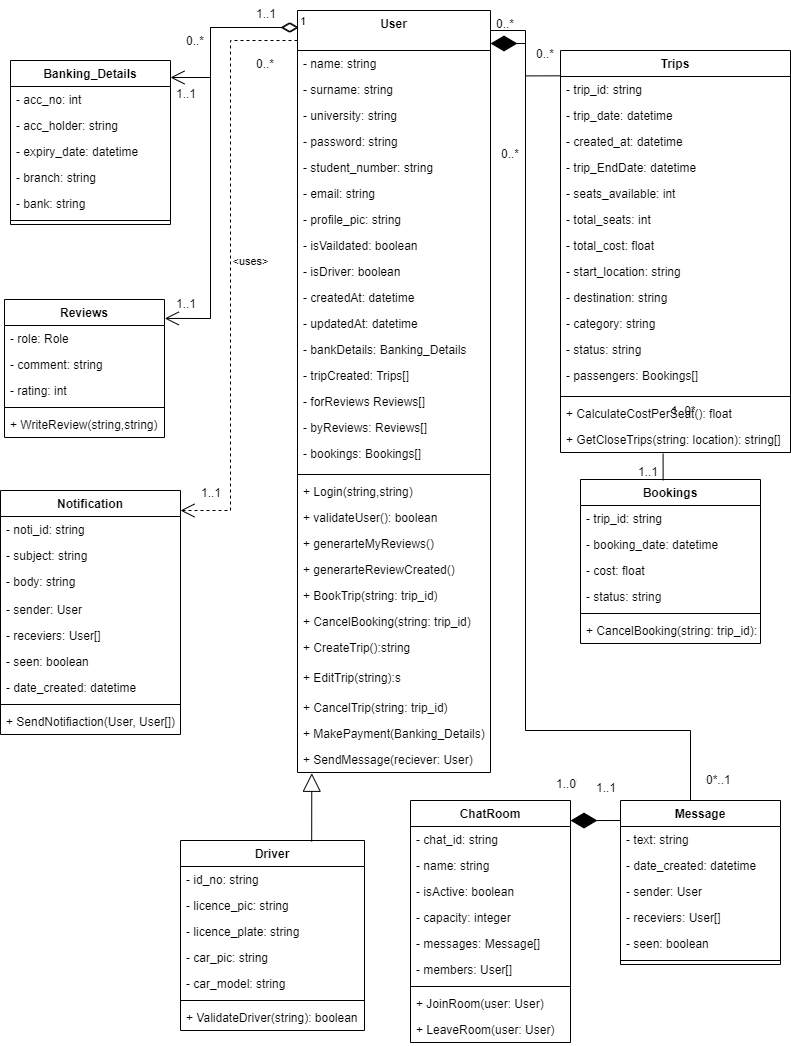
\includegraphics[scale=0.45]{images/Carpool_Class_Diagram.drawio.png}
            \caption{Carpool Class Diagram}
            \label{fig:ClassDiagram}
            
        \end{figure}
   \newpage     
        \subsection{Analysis of Class Diagram}
        
    \subsubsection{User}
        This table stores all the necessary information of the user. A user can be either a passenger, driver or both.

    \subsubsection{Banking\_Details}
       This table is responsible for storing the user’s banking details. The user can only have one bank account, and bank account can belong to only one user.
        
    \subsubsection{Reviews}
        This table stores the reviews that users leave on other user’s profiles. The role attribute refers to Driver or Passenger. A user can leave many different reviews on many different profiles, however a review can only be created by one user.
                
    
       \subsubsection{Notification table}
        This table stores all notifications that were sent either by a driver or an admin user. A notification can be sent to multiple users at the same time, however a notification can only be sent by one person.


       \subsubsection{Trips}
        This table is responsible for storing the trips that the user(driver) has created. It stores the necessary information about the trip that has been created. A user (driver) can post/ create many different trips however only one user can post/create a trip.
       
    
       \subsubsection{Booking}
        This table is responsible for storing the bookings that have been made by the user(passenger). Booking occurs when a user(passenger) requests an available seat on a trip that has been created. The booking is only confirmed once the driver has accepted their request. A user can have many bookings on many trips, however a booking can only relate to one user. A trip can have many bookings (since more then one passenger can join a trip), but a booking can only belong to one trip.
        
       \subsubsection{ChatRoom}
        This is responsible for storing information relating to a chatroom. A chatroom is created when the user confirms a booking. The chatroom allows all users that partake in the trip to send messages to one another in a central location, instead of sending messages to each user individually. A user can belong to many chatrooms, and a chatroom can have many different users.

    
      \subsubsection{Message}
        This is the actual message that is sent on the chatroom. This table stores all necessary information about the message sent as well as who sent the message, and who receives the message. A message can belong to only one chatroom, but a chatroom can consists of many different messages. A user can create many different messages, but a message can only be created/sent by one user.

    \subsubsection{Driver}
    Since a user can be both a driver and a passenger, the driver table stores all information relating to the driver. This ensures that the User table does not have null fields, since if a user is a passenger they won’t need to enter their car model and a picture of their license.
         
    
    \end{document}